\documentclass[12pt]{article}
\usepackage{baseset}
\usepackage{myproblem}
\usepackage{stackengine}
\DeclareSymbolFont{operators}{OT1}{ntxtlf}{m}{n}
\SetSymbolFont{operators}{bold}{OT1}{ntxtlf}{b}{n}
\usepackage{wasysym}
\newcommand{\RomanNumeralCaps}[1]
{\MakeUppercase{\romannumeral #1}}
\usepackage{tabularx}
\usepackage{enumitem}
\usetikzlibrary{hobby}

\begin{document}
\begin{tabularx}{\textwidth}{Xr}
{\Large \textbf{Астрофиз}} & Взлёт $09.02.2025$ \\
\end{tabularx}
\noindent\rule{\textwidth}{0.4pt}
\begin{enumerate}
    \item Вокруг звезды главной последовательности с радиусом $1.4$ радиуса Солнца и температурой $6600$ К по орбите с большой полуосью $3$ а.е. и эксцентриситетом $0.3$ обращается небольшая каменистая планета.
    \begin{enumerate}
        \item Сколько времени проходит между летним и зимним «солнцестояниями» на планете, если известно, что летнее солнцестояние в северном полушарии планеты наступает ровно в день наибольшего удаления планеты от звезды?
        \item На поверхности планеты горизонтально на почве на широте $55^{\circ}$ с. ш. установили датчик, измеряющий принятую энергию излучения, с площадью приемника $0.04$ м$^2$. Чему равна разность показаний датчика в день летнего и зимнего солнцестояний, если известно, что экватор планеты наклонен к плоскости орбиты на $23^{\circ}$?
    \end{enumerate}
    Светимость $L$ подобных звезд главной последовательности связана с их массами $M$ соотношением $l\sim M^4$.
    \item Согласно модели, используемой в статье K.P. Schroder, R.C. Smith (2008), через $12.17$ млрд лет после своего образования Солнце достигнет наибольшего размера в течение своей эволюции. Радиус Солнца будет в $256$ раз больше нынешнего, светимость станет в $2730$ раз больше нынешней, а масса уменьшится на $33.2\%$. Считайте, что потеря массы Солнцем происходит медленно в течение всей стадии красного гиганта, а физические свойства других тел Солнечной системы при росте температуры не меняются.
    Определите для момента времени, описанного выше:
    \begin{enumerate}
        \item Какие планеты Солнечной системы будут поглощены Солнцем?
        \item Найдите среднюю температуру поверхности самой горячей планеты, которая не будет поглощена Солнцем.
        \item Какие крупные тела Солнечной системы окажутся в зоне жизни (средняя температура от $250$ до $300$ K без учета парникового эффекта в атмосфере)?
    \end{enumerate}
    \item Диск далекой спиральной галактики расположен «плашмя» по отношению к лучу зрения. Характерная величина поверхностной яркости диска спиральной галактики $20^m$ с квадратной секунды. Определите характерное количество звезд в $1$ пк$^3$ диска. Межзвездным поглощением света пренебречь.
    \item В Ваше распоряжение попал наземный телескоп со специальным прибором, позволяющим разрешать видимые диски далеких звезд, если их угловой диаметр не меньше $0.02''$. Какими могут быть эффективные температуры звезд, диски которых Вы сможете различить? Атмосферные помехи и межзвездное поглощение не учитывать.
    \item Шаровое звездное скопление состоит из $500$ тысяч одинаковых звезд со светимостью, втрое меньшей солнечной. В небе Земли оно имеет звездную величину $6.0^m$ и угловой диаметр $30'$. Через некоторое время шаровое скопление пролетит сквозь диск нашей Галактики под углом $20^{\circ}$ к его плоскости. Оцените, сколько звезд солнечного типа в результате на какое-то время окажутся внутри скопления, если сейчас они расположены в диске однородно, а блеск соседней такой звезды ($\alpha$ Центавра) в нашем небе равен $0^m$. Толщина диска составляет $300$ пк, движением звезд диска, их гравитационным взаимодействием со скоплением и межзвездным поглощением света пренебречь.
    \item Ядро слабой кометы располагается в противосолнечной точке неба на расстоянии $1$ а.е. от Земли, находясь при этом в перигелии своей параболической орбиты. В этот момент в ядре происходит взрыв, разбивающий его на миллион одинаковых осколков, разлетающихся во все стороны со скоростью до $10$ м/с. Вскоре после взрыва комета на короткое время становится видимой на пределе в телескоп с диаметром объектива $8$ см. Оцените время, в течение которого комета будет превосходить по своей поверхностной яркости фон неба ($21^m$ с квадратной секунды).
    \item Оцените число фотонов в секунду, которые попадают в наш глаз от звезды класса G$2$\RomanNumeralCaps{5} с видимой звёздной величиной $m = 6^m$ при длине волны $\lambda = 550$ нм (V-диапазон). Предположите, что всё излучение этой звезды приходится на эту длину волны.
    \item Астроном на Земле наблюдает шаровое звёздное скопление с угловым диаметром $\alpha$, содержащим $N$ звёзд, каждая из которых имеет одну и ту же абсолютную звёздную величину $M_0$, и находится на расстоянии $D$ от Земли. В то же время биолог находится в центре этого скопления.
    \begin{enumerate}
        \item Какова разница между суммарными видимыми звёздными величинами всех звёзд, наблюдаемых астрономом и биологом? Считайте, что звёзды в скоплении распределены идеально равномерно, а биолог измеряет совокупную величину всего скопления.
        \item Каков должен быть диаметр телескопа астронома, если он хочет увидеть скопление с той же яркостью, что и биолог?
        \item Как будет отличаться видимая звёздная величина, наблюдаемая двумя учёными, если диаметр поля зрения биолога также равен $\alpha$?
    \end{enumerate}
    \item Красная и оранжевая звезды составляют затменную двойную систему. Красная звезда на $0.5^m$ ярче оранжевой, а ее радиус в $2.6$ раза больше. Определите падение блеска двойной в главном и вторичном минимуме, если затмения в системе центральные. Чему равно отношение температур звезд? Потемнением дисков звезд к краю пренебречь.
    \item Перед Вами кривые блеска пяти переменных звезд (следующая страница). Соотнесите их с пятью типами переменных A-E и поставьте соответствующие буквы на листе ответов. Известно, что каждый тип переменности представлен один раз.
    A: Пульсирующая переменная горизонтальной ветви, масса -- не более массы Солнца. Период пульсации -- от нескольких часов до нескольких суток.

    B: Два компонента образуют контактную двойную, возможно перетекание вещества с одного компонента на другой. Луч зрения наблюдателя лежит в плоскости относительной орбиты звезд. Температуры компонентов практически одинаковы, возможно наличие общей оболочки.

    C: Пульсирующая переменная (цефеида) первого типа звездного населения.

    D: Два компонента почти сферически-симметричны и отделены друг от друга. Температуры звезд заметно различаются. Луч зрения наблюдателя лежит в плоскости относительной орбиты звезд.

    E: Компонентами двойной системы являются красный гигант и массивный белый карлик. Переменность звезды вызвана аккрецией вещества на белый карлик с последующими взрывоподобными процессами.
    \begin{figure}[h]
        \centering
        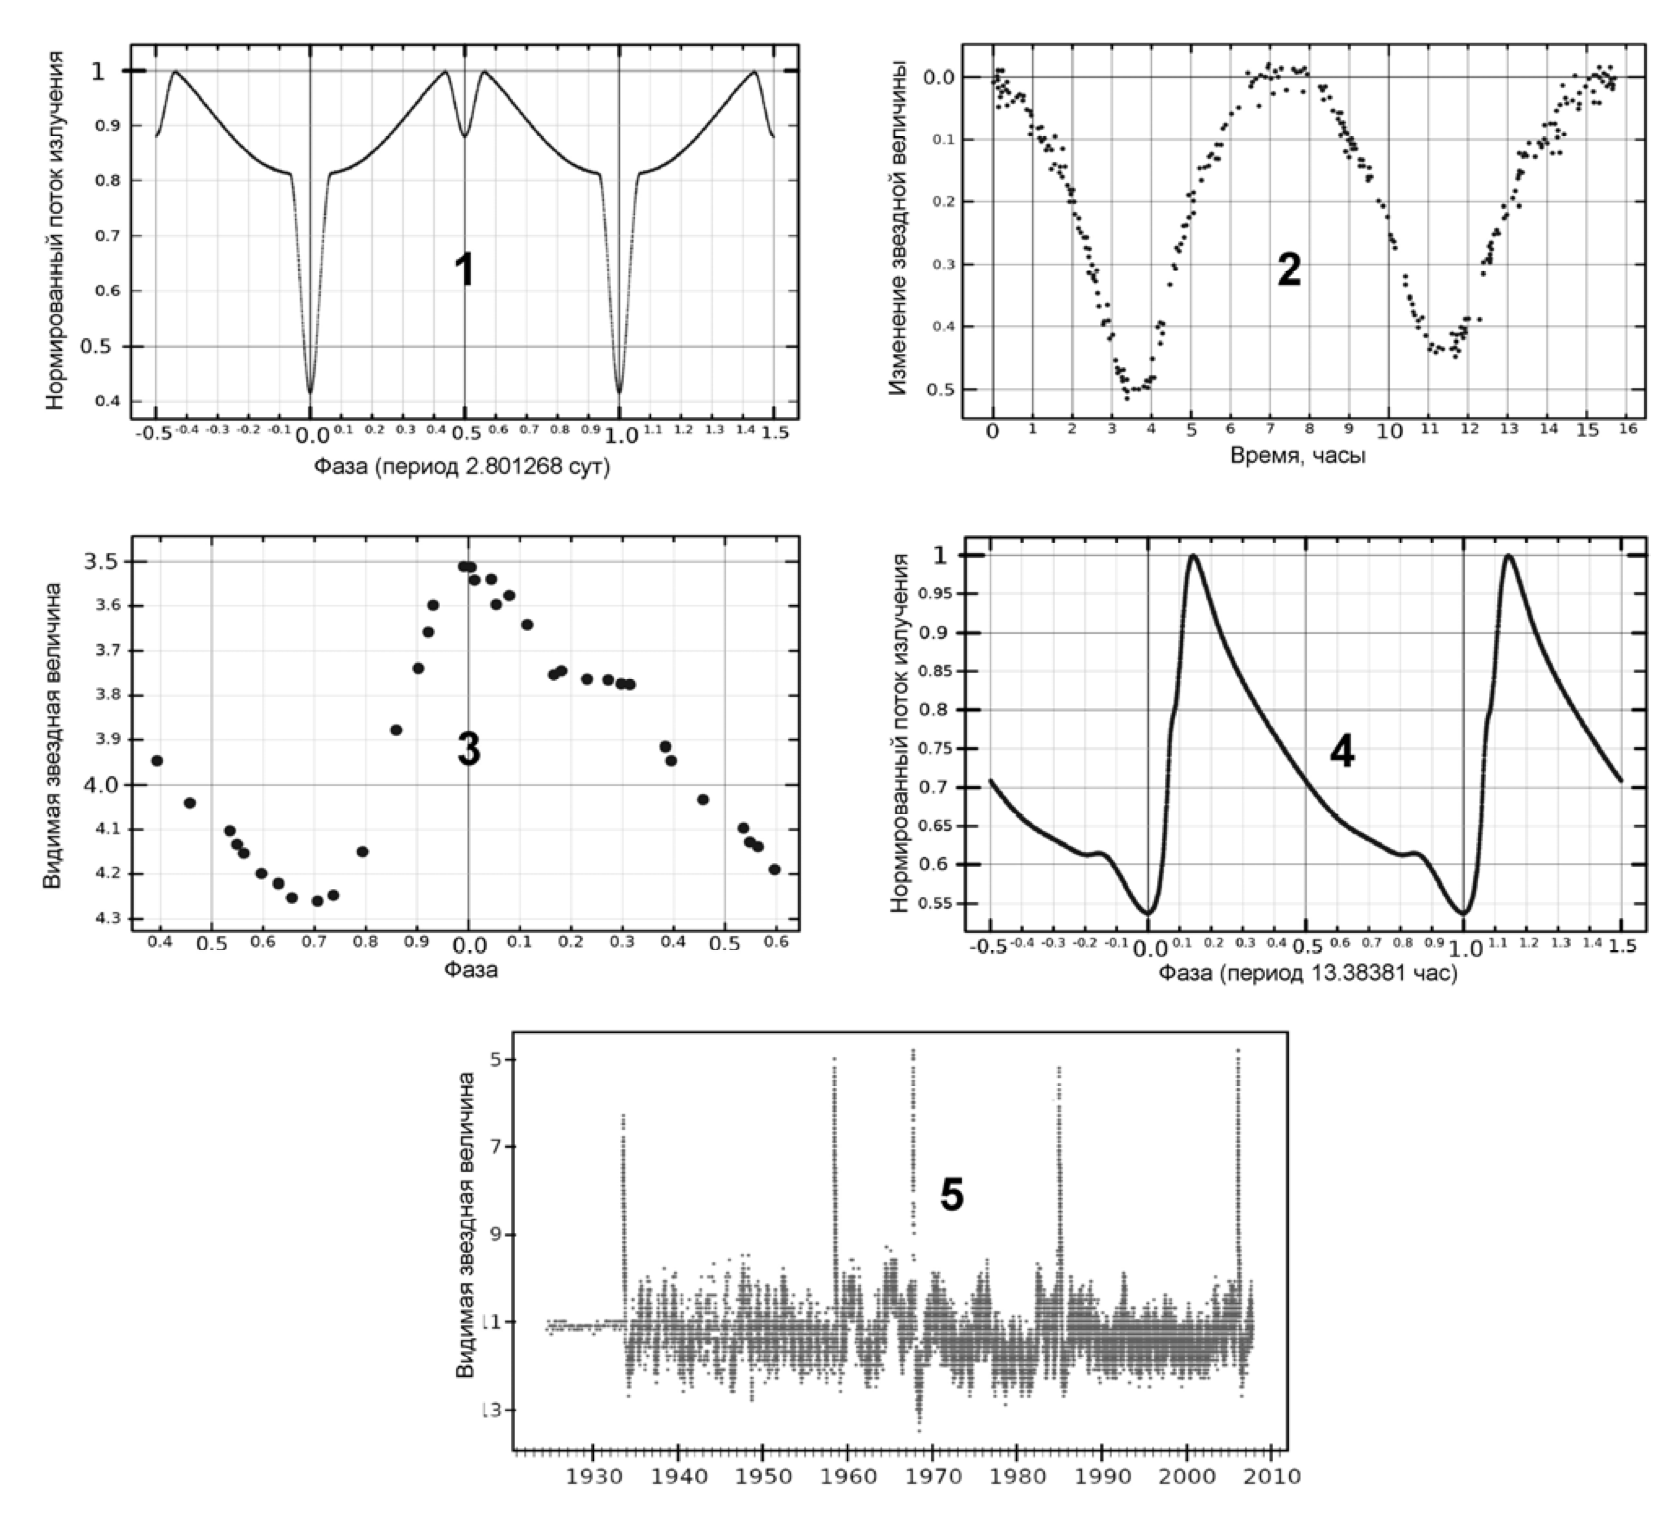
\includegraphics[width = \textwidth]{curves1.png}
    \end{figure}
    \item Перед Вами кривые блеска некоторых звезд: с пятном на экваторе (A); с пятном в высоких широтах (B); с планетой, проходящей по центру видимого диска звезды (C); с планетой, проходящей по короткои хорде (D). Расставьте буквы A, B, C и D напротив цифр 1, 2, 3 и 4; известно, что каждая буква встречается в ответе один раз.
    По оси абсцисс отложена орбитальная фаза ($t/T$, где $t$ -- время, T -- период вращения звезды с пятном или планеты), вертикальный масштаб четырех графиков (звездные величины) может различаться. Пятно имеет круглую форму с постоянным радиусом, звезды и планеты -- сферические. Орбиты планет – круговые. Пятно движется только вместе с вращающейся звездой, не перемещаясь по ее поверхности и не меняя размер. Радиус планеты и пятна в несколько раз меньше радиуса звезды. Во всех случаях наблюдатель находится в плоскости экватора звезды. Потемнение звезд к краю не учитывать.
    \begin{figure}[h]
        \centering
        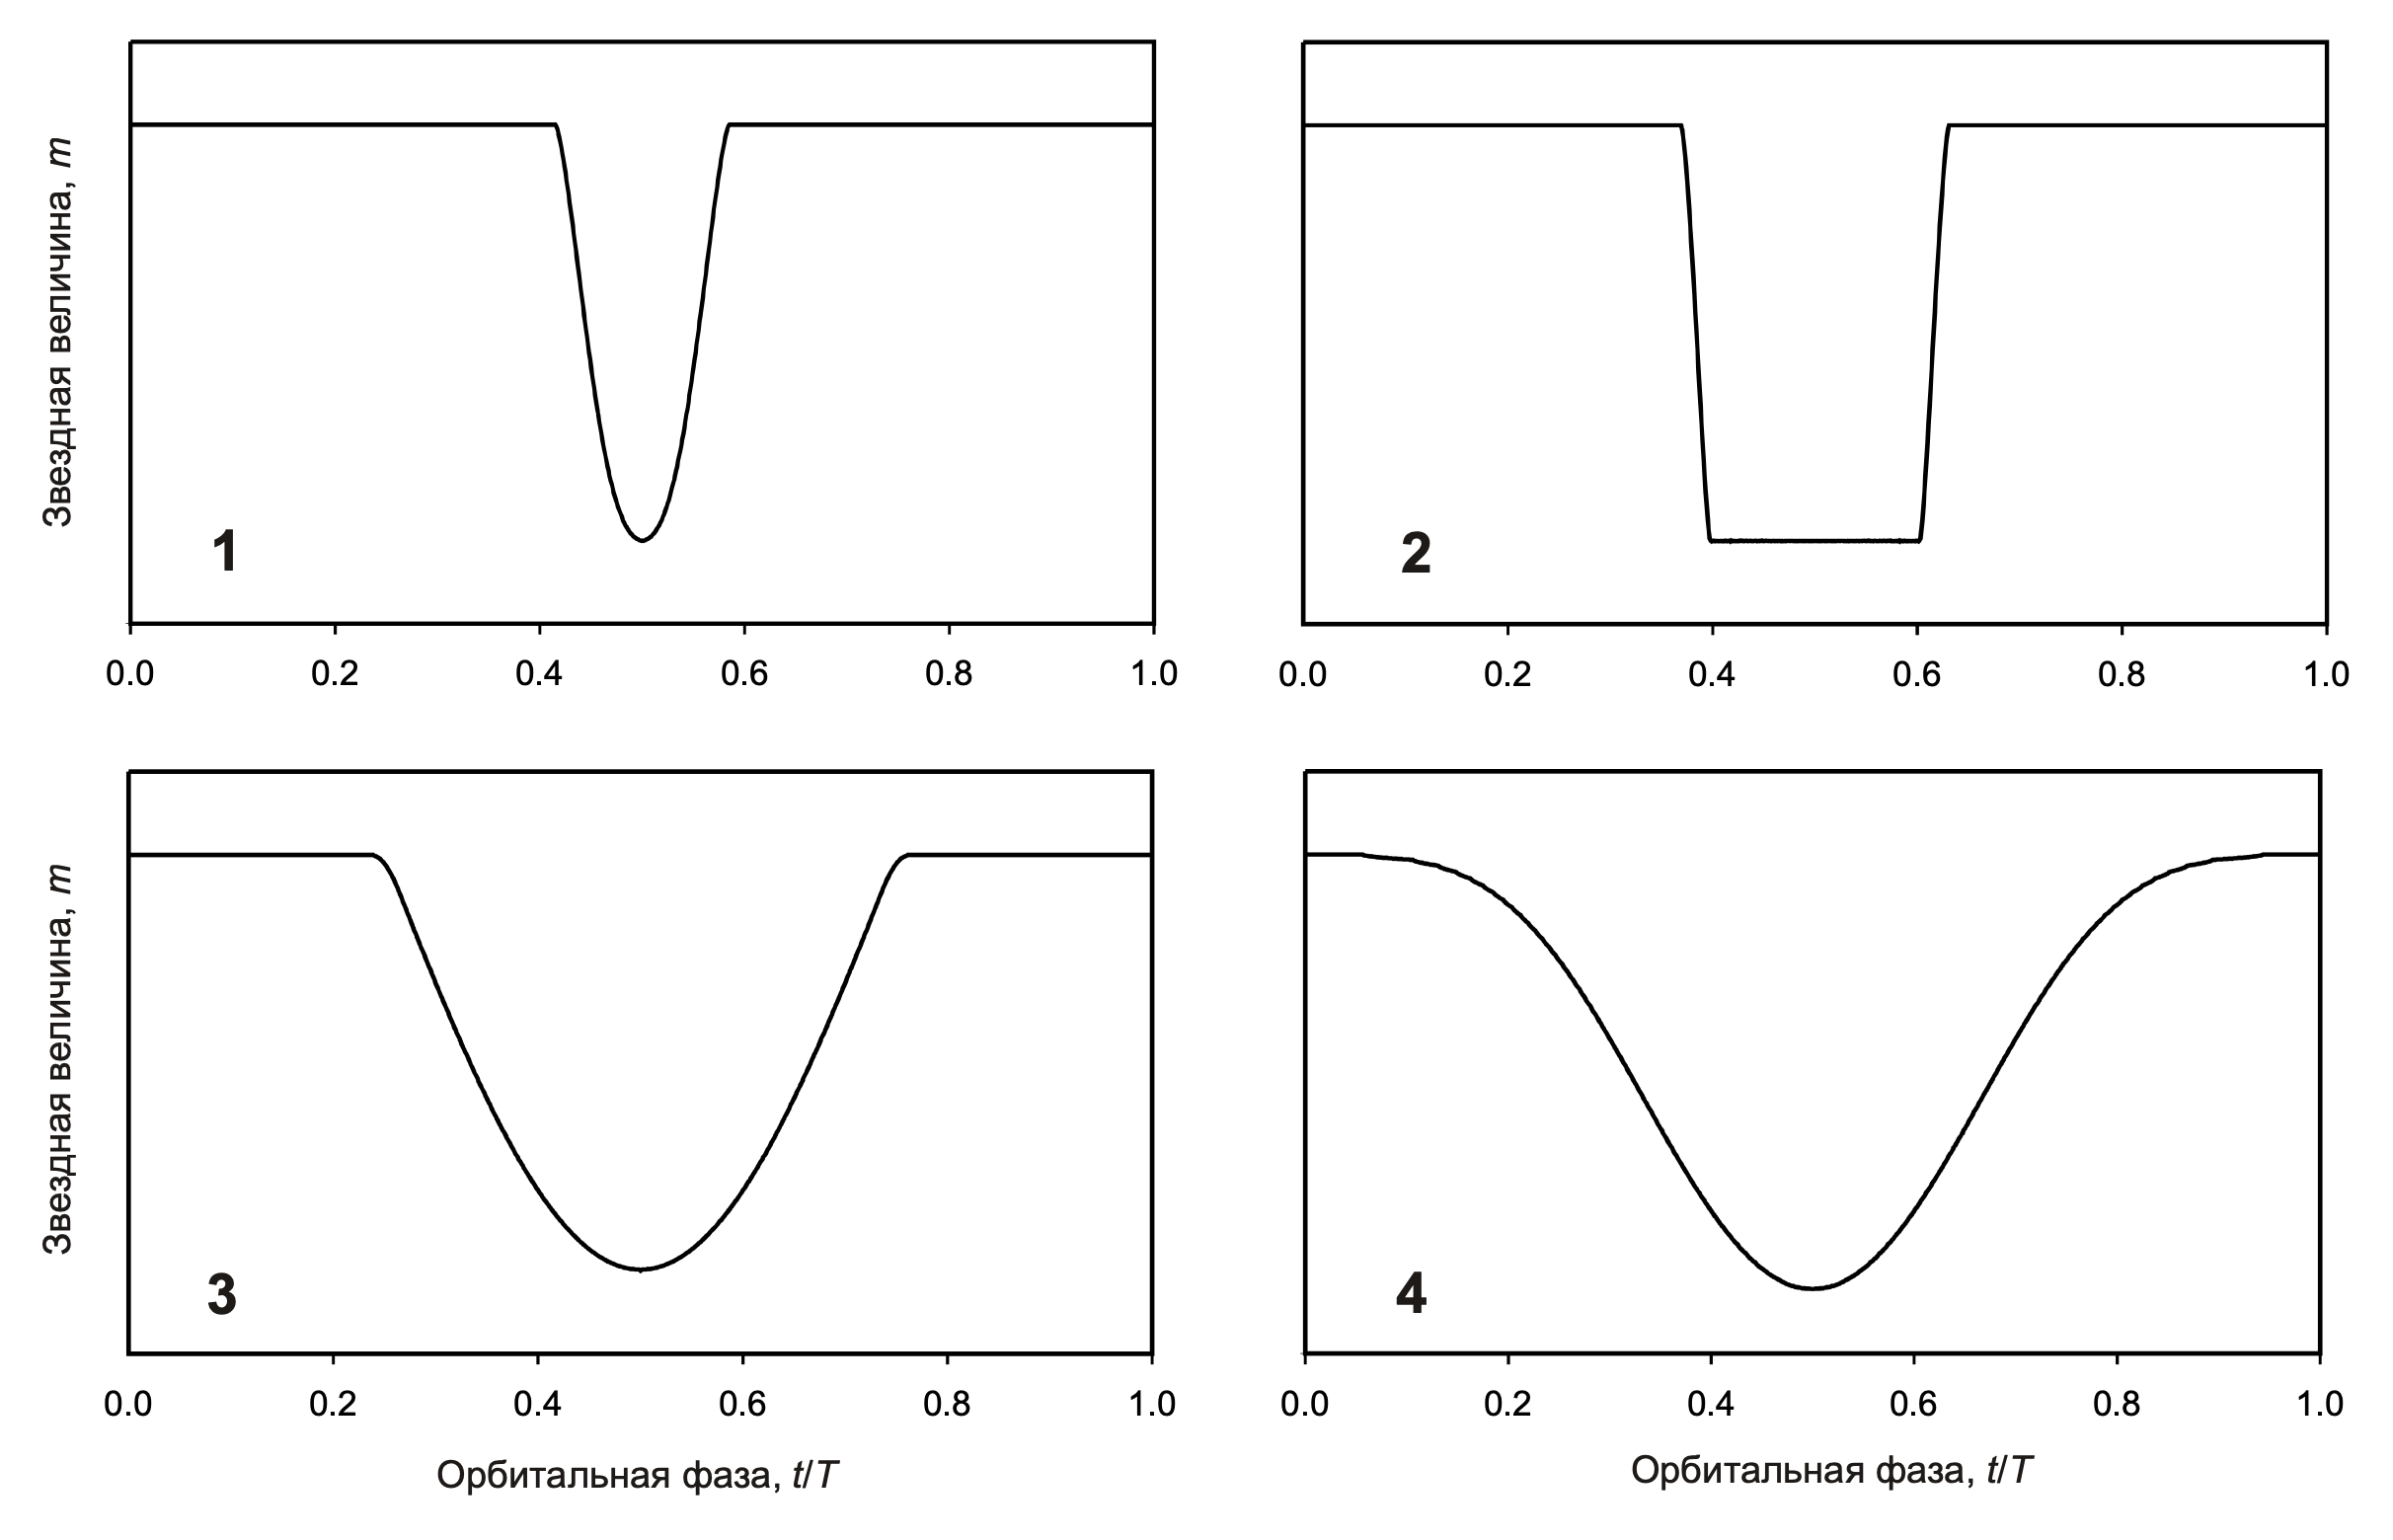
\includegraphics[width = \textwidth]{curves2.png}
    \end{figure}
    \item На каком примерно расстоянии надо поместить $75$-ваттную лампочку дневного света (КПД = $10\%$), чтобы она имела блеск $0^m$ в тумане с коэффициентом рассеяния $1^m$/км?
    \item В Галактике Млечный Путь раз в $20$ лет вспыхивают Сверхновые \RomanNumeralCaps{2} типа с абсолютной звездной величиной $-18^m$. Насколько часто такие Сверхновые по- являются в небе Земли с блеском ярче Венеры ($-4^m$)? Радиус Галактики считать равным $15$ кпк, поглощение света составляет $2^m$/кпк.
    \item На рисунке приведена кривая блеска  затменно-переменной звезды. Определите по графику соотношения светимостей, радиусов и температур звезд.
       \begin{figure}[h] 	
           \centering
           \begin{tikzpicture} 
           \begin{axis}[xlabel=время,
           ylabel=звездная величина, 
           grid=major, 
           y dir=reverse, 
           width=10cm, 
           legend pos = south west,
           ymax=3.5]
           \addplot[line width=1pt, black] coordinates {
               (0, 2.5)
               (1, 2.5)
               (1.9, 3.1)
               (2.1, 3.1)
               (3, 2.5)
               %(4, 2)
               (4, 2.5)
               (4.9, 3.3)
               (5.1, 3.3)
               (6, 2.5)
               (7, 2.5)
               (7.9, 3.1)
               (8.1, 3.1)
               (9, 2.5)
               (10, 2.5)
               %(12, 2)
               (10.9, 3.3)
               (11.1, 3.3)
               (12, 2.5)
               (13, 2.5)
           };
       
           \end{axis}
           \end{tikzpicture} 
       \end{figure}
       \item Фотометрические наблюдения, позволили построить интегральную кривую блеска двойной системы (по вертикальной оси отложен поток), на которой оказалось два минимума. Чему равно отношение эффективных температур звезд, если первичный минимум в $2$ раза  глубже вторичного?
       %\documentclass[a5paper]{article}
%\usepackage[russian]{babel}
%%\usepackage[left=1cm,right=1cm,top=1cm,bottom=2cm,bindingoffset=0cm]{geometry}
%\usepackage{geometry}
%\usepackage{graphicx}
%\usepackage{multirow}
%\usepackage{array}
%\usepackage{pgfplots}	
%\usepackage{amssymb}
%\usepackage{mathrsfs}
%\usepackage{autonum}
%\usepackage{amsmath}
%\usepackage{wrapfig}
%\usepackage{floatflt}
%\usepackage{wasysym}
%\usepackage{tkz-euclide}
% \usetikzlibrary{hobby}
% \usetikzlibrary{intersections, spath3}
%
%\begin{document}
%
%
%\enlargethispage{\baselineskip}
%\newpage
%

%\begin{center}
\begin{figure}[h]
\centering
\begin{tikzpicture}[scale=1.2, use Hobby shortcut,
 tangent/.style={%
  in angle={(180+#1)} ,
  Hobby finish ,
  designated Hobby path=next , out angle=#1,
 }, dot/.style = {draw, fill = black, color = black, circle, inner sep=1pt}, scale = 1.4]
 \coordinate (O) at (0,0);
 \coordinate (Y) at (0, 2.2);
 \coordinate (X) at (6.49, 0);
 
 \coordinate[label = above left:{$I$}] (rentlabel) at (Y);


 \draw (-0.45,1.7) -- node[ left=0.9mm] {$2 \Delta I$} (-0.45,0.655069631546032);
 \draw[white,line width=0.5mm] (-0.45,1.7) -- (-0.45,0.655069631546032);

 \draw  [decorate,decoration={brace,amplitude=4pt,mirror}] (0,1.7)--(0,1.17757079316651);
 \draw (0,1.17757079316651) -- node[ left=0.9mm] {$\Delta I$} (0,1.7);

 \draw  [decorate,decoration={brace,amplitude=4pt,mirror}] (-0.45,1.7)--(-0.45,0.655069631546032);






 \draw[dashed,gray] (0.99999,0.655069631546032) -- (-0.45,0.655069631546032);
 \draw[dashed,gray] (-0.45,1.7) -- (0,1.7);

 \draw[dashed,gray] (2.99999,1.17757079316651) -- (0,1.17757079316651);

 \draw[-latex] (O) -- (Y);
 \draw[-latex] (O) -- (X);





 \coordinate[label = below:{\small Фаза}] (timelable) at (X);
 
 \draw (1,-0.05) -- (1,0.08);

 \coordinate[label = below:{\small 0}] (0) at (1, 0);

 \draw (3,-0.05) -- (3,0.1);

 \coordinate[label = below:{\small 0.5}] (0.5) at (3, 0);

 \draw (5,-0.05) -- (5,0.1);

 \coordinate[label = below:{\small 1}] (1) at (5, 0);







 \draw[line width=0.25mm] (0,1.7) -- (0.5,1.7);

 
 \draw[line width=0.25mm] (0.5,1.7) .. 
 (0.5049999,1.69919540924519) .. 
 (0.5099998,1.69772616391491) .. 
 (0.5149997,1.69582535847761) .. 
 (0.5199996,1.69357581820984) .. 
 (0.5249995,1.69102506785595) .. 
 (0.5299994,1.68820486947486) .. 
 (0.5349993,1.6851382710901) .. 
 (0.5399992,1.68184288905459) .. 
 (0.5449991,1.67833267750399) .. 
 (0.549999,1.67461897955738) .. 
 (0.5549989,1.67071119697222) .. 
 (0.5599988,1.66661723987201) .. 
 (0.5649987,1.66234384154679) .. 
 (0.5699986,1.65789678628655) .. 
 (0.5749985,1.65328107886571) .. 
 (0.5799984,1.64850107355402) .. 
 (0.5849983,1.64356057425248) .. 
 (0.5899982,1.638462913527) .. 
 (0.5949981,1.63321101589496) .. 
 (0.599998,1.62780744914384) .. 
 (0.6049979,1.62225446640571) .. 
 (0.6099978,1.61655404098801) .. 
 (0.6149977,1.61070789545353) .. 
 (0.6199976,1.60471752608129) .. 
 (0.6249975,1.59858422357713) .. 
 (0.6299974,1.59230909070917) .. 
 (0.6349973,1.58589305739901) .. 
 (0.6399972,1.57933689368954) .. 
 (0.6449971,1.57264122092678) .. 
 (0.649997,1.56580652142803) .. 
 (0.6549969,1.55883314685789) .. 
 (0.6599968,1.55172132549375) .. 
 (0.6649967,1.54447116853028) .. 
 (0.6699966,1.53708267554705) .. 
 (0.6749965,1.5295557392427) .. 
 (0.6799964,1.521890149522) .. 
 (0.6849963,1.51408559700864) .. 
 (0.6899962,1.50614167604497) .. 
 (0.6949961,1.4980578872304) .. 
 (0.699996,1.4898336395424) .. 
 (0.7049959,1.48146825207711) .. 
 (0.7099958,1.47296095544119) .. 
 (0.7149957,1.46431089282136) .. 
 (0.7199956,1.45551712075435) .. 
 (0.7249955,1.44657860961598) .. 
 (0.7299954,1.43749424384521) .. 
 (0.7349953,1.42826282191624) .. 
 (0.7399952,1.41888305606925) .. 
 (0.7449951,1.40935357180818) .. 
 (0.749995,1.39967290717211) .. 
 (0.7549949,1.3898395117849) .. 
 (0.7599948,1.37985174568628) .. 
 (0.7649947,1.36970787794582) .. 
 (0.7699946,1.35940608505998) .. 
 (0.7749945,1.34894444913108) .. 
 (0.7799944,1.3383209558255) .. 
 (0.7849943,1.32753349210746) .. 
 (0.7899942,1.31657984374309) .. 
 (0.7949941,1.30545769256869) .. 
 (0.799994,1.29416461351525) .. 
 (0.8049939,1.28269807138051) .. 
 (0.8099938,1.27105541733824) .. 
 (0.8149937,1.25923388517288) .. 
 (0.8199936,1.24723058722663) .. 
 (0.8249935,1.23504251004408) .. 
 (0.8299934,1.22266650969815) .. 
 (0.8349933,1.21009930677912) .. 
 (0.8399932,1.19733748102691) .. 
 (0.8449931,1.18437746558437) .. 
 (0.849993,1.17121554084751) .. 
 (0.8549929,1.15784782788595) .. 
 (0.8599928,1.14427028140442) .. 
 (0.8649927,1.13047868221303) .. 
 (0.8699926,1.11646862917143) .. 
 (0.8749925,1.10223553056782) .. 
 (0.8799924,1.08777459489067) .. 
 (0.8849923,1.07308082094645) .. 
 (0.8899922,1.05814898727212) .. 
 (0.8949921,1.04297364078619) .. 
 (0.899992,1.02754908461619) .. 
 (0.9049919,1.01186936503456) .. 
 (0.9099918,0.99592825742742) .. 
 (0.9149917,0.97971925121323) .. 
 (0.9199916,0.96323553361961) .. 
 (0.9249915,0.94646997221643) .. 
 (0.9299914,0.92941509609293) .. 
 (0.9349913,0.91206307555357) .. 
 (0.9399912,0.89440570019409) .. 
 (0.9449911,0.87643435520316) .. 
 (0.949991,0.85813999571741) .. 
 (0.9549909,0.83951311903782) .. 
 (0.9599908,0.82054373449232) .. 
 (0.9649907,0.80122133070393) .. 
 (0.9699906,0.78153483999419) .. 
 (0.9749905,0.761472599618) .. 
 (0.9799904,0.7410223094875) .. 
 (0.9849903,0.7201709859986) .. 
 (0.9899902,0.698904911522729) .. 
 (0.9949901,0.677209579068137) .. 
 (0.99999,0.655069631546032);


 \draw[line width=0.25mm] (1,0.6550696315) .. 
(1.005,0.677166185616169) .. 
(1.01,0.698862812551183) .. 
(1.015,0.7201301350844) .. 
(1.02,0.7409826626752) .. 
(1.025,0.76143411524417) .. 
(1.03,0.7814974785272) .. 
(1.035,0.8011850545975) .. 
(1.04,0.8205085080515) .. 
(1.045,0.83947890829609) .. 
(1.05,0.8581067683238) .. 
(1.055,0.8764020803185) .. 
(1.06,0.89437434839543) .. 
(1.065,0.91203261874602) .. 
(1.07,0.92938550742829) .. 
(1.075,0.94644122601797) .. 
(1.08,0.96320760531234) .. 
(1.085,0.9796921172594) .. 
(1.09,0.99590189526653) .. 
(1.095,1.01184375302773) .. 
(1.1,1.02752420199435) .. 
(1.105,1.04294946760186) .. 
(1.11,1.05812550435449) .. 
(1.115,1.07305800985938) .. 
(1.12,1.08775243789357) .. 
(1.125,1.10221401057898) .. 
(1.13,1.11644772973375) .. 
(1.135,1.13045838746189) .. 
(1.14,1.14425057603754) .. 
(1.145,1.15782869713518) .. 
(1.15,1.1711969704522) .. 
(1.155,1.18435944176644) .. 
(1.16,1.19731999046732) .. 
(1.165,1.21008233659575) .. 
(1.17,1.2226500474249) .. 
(1.175,1.23502654361121) .. 
(1.18,1.24721510494212) .. 
(1.185,1.25921887570487) .. 
(1.19,1.27104086969838) .. 
(1.195,1.28268397490823) .. 
(1.2,1.29415095786279) .. 
(1.205,1.30544446768699) .. 
(1.21,1.31656703986831) .. 
(1.215,1.32752109974821) .. 
(1.22,1.33830896575071) .. 
(1.225,1.3489328523584) .. 
(1.23,1.35939487284478) .. 
(1.235,1.36969704177067) .. 
(1.24,1.37984127725089) .. 
(1.245,1.38982940299654) .. 
(1.25,1.39966315013641) .. 
(1.255,1.40934415882034) .. 
(1.26,1.41887397960557) .. 
(1.265,1.42825407462603) .. 
(1.27,1.43748581854296) .. 
(1.275,1.44657049927387) .. 
(1.28,1.45550931849497) .. 
(1.285,1.4643033919107) .. 
(1.29,1.47295374928185) .. 
(1.295,1.48146133420171) .. 
(1.3,1.48982700360717) .. 
(1.305,1.49805152700895) .. 
(1.31,1.50613558542215) .. 
(1.315,1.51407976997462) .. 
(1.32,1.52188458016636) .. 
(1.325,1.52955042174866) .. 
(1.33,1.53707760418573) .. 
(1.335,1.54446633765507) .. 
(1.34,1.55171672953464) .. 
(1.345,1.55882878031579) .. 
(1.35,1.56580237886913) .. 
(1.355,1.5726372969768) .. 
(1.36,1.5793331830279) .. 
(1.365,1.58588955475291) .. 
(1.37,1.59230579084746) .. 
(1.375,1.59858112130405) .. 
(1.38,1.6047146162299) .. 
(1.385,1.61070517287885) .. 
(1.39,1.61655150055979) .. 
(1.395,1.62225210300074) .. 
(1.4,1.6278052576377) .. 
(1.405,1.63320899115311) .. 
(1.41,1.63846105039502) .. 
(1.415,1.64355886754541) .. 
(1.42,1.6484995180444) .. 
(1.425,1.65327966927014) .. 
(1.43,1.65789551725046) .. 
(1.435,1.66234270762678) .. 
(1.44,1.66661623551531) .. 
(1.445,1.67071031649221) .. 
(1.45,1.67461821710413) .. 
(1.455,1.67833202702788) .. 
(1.46,1.6818423442605) .. 
(1.465,1.68513782537811) .. 
(1.47,1.68820451586067) .. 
(1.475,1.69102479885975) .. 
(1.48,1.69357562569176) .. 
(1.485,1.69582523337434) .. 
(1.49,1.69772609576412) .. 
(1.495,1.69919538512214) .. 
(1.5,1.7);

\draw[line width=0.25mm] (1.5,1.7) -- (2.5,1.7);

\draw[line width=0.25mm] (2.5,1.7) .. 
(2.5049999,1.69950283329736) .. 
(2.5099998,1.69859533149484) .. 
(2.5149997,1.6974219667914) .. 
(2.5199996,1.69603434450002) .. 
(2.5249995,1.69446225469984) .. 
(2.5299994,1.69272574746573) .. 
(2.5349993,1.6908394896682) .. 
(2.5399992,1.68881479413853) .. 
(2.5449991,1.686660713805) .. 
(2.549999,1.68438469191274) .. 
(2.5549989,1.68199297642149) .. 
(2.5599988,1.67949089846861) .. 
(2.5649987,1.67688306743258) .. 
(2.5699986,1.6741735122407) .. 
(2.5749985,1.67136578661045) .. 
(2.5799984,1.66846304927446) .. 
(2.5849983,1.66546812635947) .. 
(2.5899982,1.66238356072516) .. 
(2.5949981,1.65921165157414) .. 
(2.599998,1.65595448667062) .. 
(2.6049979,1.65261396885265) .. 
(2.6099978,1.64919183807565) .. 
(2.6149977,1.64568968991158) .. 
(2.6199976,1.64210899120439) .. 
(2.6249975,1.6384510934201) .. 
(2.6299974,1.63471724411023) .. 
(2.6349973,1.63090859681795) .. 
(2.6399972,1.62702621968846) .. 
(2.6449971,1.6230711029935) .. 
(2.649997,1.61904416573965) .. 
(2.6549969,1.61494626149888) .. 
(2.6599968,1.61077818357493) .. 
(2.6649967,1.6065406695996) .. 
(2.6699966,1.60223440563712) .. 
(2.6749965,1.59786002986226) .. 
(2.6799964,1.59341813586721) .. 
(2.6849963,1.58890927564409) .. 
(2.6899962,1.58433396228274) .. 
(2.6949961,1.57969267241779) .. 
(2.699996,1.57498584845426) .. 
(2.7049959,1.57021390059666) .. 
(2.7099958,1.56537720870365) .. 
(2.7149957,1.56047612398688) .. 
(2.7199956,1.55551097057073) .. 
(2.7249955,1.55048204692729) .. 
(2.7299954,1.54538962719936) .. 
(2.7349953,1.54023396242251) .. 
(2.7399952,1.53501528165621) .. 
(2.7449951,1.52973379303267) .. 
(2.749995,1.52438968473129) .. 
(2.7549949,1.51898312588558) .. 
(2.7599948,1.51351426742871) .. 
(2.7649947,1.50798324288335) .. 
(2.7699946,1.50239016910077) .. 
(2.7749945,1.49673514695364) .. 
(2.7799944,1.4910182619866) .. 
(2.7849943,1.48523958502842) .. 
(2.7899942,1.47939917276891) .. 
(2.7949941,1.47349706830369) .. 
(2.799994,1.46753330164973) .. 
(2.8049939,1.46150789023398) .. 
(2.8099938,1.45542083935756) .. 
(2.8149937,1.44927214263774) .. 
(2.8199936,1.44306178242945) .. 
(2.8249935,1.43678973022841) .. 
(2.8299934,1.43045594705746) .. 
(2.8349933,1.42406038383772) .. 
(2.8399932,1.41760298174602) .. 
(2.8449931,1.41108367256007) .. 
(2.849993,1.40450237899266) .. 
(2.8549929,1.3978590150161) .. 
(2.8599928,1.39115348617813) .. 
(2.8649927,1.38438568991038) .. 
(2.8699926,1.3775555158305) .. 
(2.8749925,1.37066284603897) .. 
(2.8799924,1.3637075554116) .. 
(2.8849923,1.35668951188865) .. 
(2.8899922,1.34960857676158) .. 
(2.8949921,1.34246460495831) .. 
(2.899992,1.33525744532788) .. 
(2.9049919,1.32798694092545) .. 
(2.9099918,1.32065292929848) .. 
(2.9149917,1.31325524277503) .. 
(2.9199916,1.30579370875499) .. 
(2.9249915,1.29826815000516) .. 
(2.9299914,1.29067838495914) .. 
(2.9349913,1.28302422802278) .. 
(2.9399912,1.27530548988628) .. 
(2.9449911,1.26752197784372) .. 
(2.949991,1.25967349612111) .. 
(2.9549909,1.25175984621382) .. 
(2.9599908,1.24378082723452) .. 
(2.9649907,1.23573623627253) .. 
(2.9699906,1.2276258687658) .. 
(2.9749905,1.21944951888647) .. 
(2.9799904,1.21120697994136) .. 
(2.9849903,1.20289804478837) .. 
(2.9899902,1.19452250627021) .. 
(2.9949901,1.1860801576667) .. 
(2.99999,1.17757079316651);

\draw[line width=0.25mm] (3,1.177570793) .. 
(3.005,1.18606337507142) .. 
(3.01,1.19450602435027) .. 
(3.015,1.20288186046682) .. 
(3.02,1.21119109015236) .. 
(3.025,1.2194339205762) .. 
(3.03,1.2276105588933) .. 
(3.035,1.23572121181052) .. 
(3.04,1.24376608517003) .. 
(3.045,1.25174538354888) .. 
(3.05,1.25965930987327) .. 
(3.055,1.26750806504659) .. 
(3.06,1.27529184758995) .. 
(3.065,1.28301085329422) .. 
(3.07,1.29066527488253) .. 
(3.075,1.29825530168222) .. 
(3.08,1.30578111930517) .. 
(3.085,1.31324290933575) .. 
(3.09,1.32064084902528) .. 
(3.095,1.32797511099211) .. 
(3.1,1.33524586292653) .. 
(3.105,1.34245326729943) .. 
(3.11,1.34959748107408) .. 
(3.115,1.35667865541982) .. 
(3.12,1.36369693542707) .. 
(3.125,1.37065245982265) .. 
(3.13,1.37754536068447) .. 
(3.135,1.3843757631548) .. 
(3.14,1.39114378515104) .. 
(3.145,1.3978495370733) .. 
(3.15,1.40449312150747) .. 
(3.155,1.41107463292315) .. 
(3.16,1.41759415736512) .. 
(3.165,1.42405177213741) .. 
(3.17,1.43044754547888) .. 
(3.175,1.43678153622893) .. 
(3.18,1.44305379348241) .. 
(3.185,1.44926435623206) .. 
(3.19,1.45541325299743) .. 
(3.195,1.46150050143846) .. 
(3.2,1.46752610795238) .. 
(3.205,1.47349006725213) .. 
(3.21,1.47939236192443) .. 
(3.215,1.48523296196553) .. 
(3.22,1.49101182429253) .. 
(3.225,1.49672889222789) .. 
(3.23,1.50238409495461) .. 
(3.235,1.50797734693925) .. 
(3.24,1.51350854731985) .. 
(3.245,1.51897757925526) .. 
(3.25,1.52438430923234) .. 
(3.255,1.52972858632682) .. 
(3.26,1.53501024141348) .. 
(3.265,1.54022908632053) .. 
(3.27,1.54538491292266) .. 
(3.275,1.55047749216661) .. 
(3.28,1.55550657302222) .. 
(3.285,1.56047188135136) .. 
(3.29,1.56537311868573) .. 
(3.295,1.57020996090389) .. 
(3.3,1.57498205679623) .. 
(3.305,1.57968902650518) .. 
(3.31,1.58433045982626) .. 
(3.315,1.58890591435347) .. 
(3.32,1.59341491345004) .. 
(3.325,1.59785694402282) .. 
(3.33,1.6022314540751) .. 
(3.335,1.60653785000876) .. 
(3.34,1.61077549364166) .. 
(3.345,1.61494369890066) .. 
(3.35,1.61904172814343) .. 
(3.355,1.62306878805391) .. 
(3.36,1.62702402504591) .. 
(3.365,1.63090652009657) .. 
(3.37,1.63471528291564) .. 
(3.375,1.63844924533698) .. 
(3.38,1.64210725379381) .. 
(3.385,1.64568806070806) .. 
(3.39,1.64919031458399) .. 
(3.395,1.65261254854434) .. 
(3.4,1.65595316697986) .. 
(3.405,1.65921042989342) .. 
(3.41,1.66238243440025) .. 
(3.415,1.66546709268377) .. 
(3.42,1.66846210548252) .. 
(3.425,1.67136492987052) .. 
(3.43,1.67417273964611) .. 
(3.435,1.6768823759916) .. 
(3.44,1.67949028509241) .. 
(3.445,1.68199243790972) .. 
(3.45,1.68438422493589) .. 
(3.455,1.68666031488247) .. 
(3.46,1.68881445961085) .. 
(3.465,1.69083921566081) .. 
(3.47,1.69272552984024) .. 
(3.475,1.69446208898564) .. 
(3.48,1.69603422579295) .. 
(3.485,1.69742188959119) .. 
(3.49,1.69859528941136) .. 
(3.495,1.69950281839354) .. 
(3.5,1.7);

\draw[line width=0.25mm] (3.5,1.7) -- (4.5,1.7);

\draw[line width=0.25mm] (4.5,1.7) .. 
(4.5049999,1.69919540924519) .. 
(4.5099998,1.69772616391491) .. 
(4.5149997,1.69582535847761) .. 
(4.5199996,1.69357581820984) .. 
(4.5249995,1.69102506785595) .. 
(4.5299994,1.68820486947486) .. 
(4.5349993,1.6851382710901) .. 
(4.5399992,1.68184288905459) .. 
(4.5449991,1.67833267750399) .. 
(4.549999,1.67461897955738) .. 
(4.5549989,1.67071119697222) .. 
(4.5599988,1.66661723987201) .. 
(4.5649987,1.66234384154679) .. 
(4.5699986,1.65789678628655) .. 
(4.5749985,1.65328107886571) .. 
(4.5799984,1.64850107355402) .. 
(4.5849983,1.64356057425248) .. 
(4.5899982,1.638462913527) .. 
(4.5949981,1.63321101589496) .. 
(4.599998,1.62780744914384) .. 
(4.6049979,1.62225446640571) .. 
(4.6099978,1.61655404098801) .. 
(4.6149977,1.61070789545353) .. 
(4.6199976,1.60471752608129) .. 
(4.6249975,1.59858422357713) .. 
(4.6299974,1.59230909070917) .. 
(4.6349973,1.58589305739901) .. 
(4.6399972,1.57933689368954) .. 
(4.6449971,1.57264122092678) .. 
(4.649997,1.56580652142803) .. 
(4.6549969,1.55883314685789) .. 
(4.6599968,1.55172132549375) .. 
(4.6649967,1.54447116853028) .. 
(4.6699966,1.53708267554705) .. 
(4.6749965,1.5295557392427) .. 
(4.6799964,1.521890149522) .. 
(4.6849963,1.51408559700864) .. 
(4.6899962,1.50614167604497) .. 
(4.6949961,1.4980578872304) .. 
(4.699996,1.4898336395424) .. 
(4.7049959,1.48146825207711) .. 
(4.7099958,1.47296095544119) .. 
(4.7149957,1.46431089282136) .. 
(4.7199956,1.45551712075435) .. 
(4.7249955,1.44657860961598) .. 
(4.7299954,1.43749424384521) .. 
(4.7349953,1.42826282191624) .. 
(4.7399952,1.41888305606925) .. 
(4.7449951,1.40935357180818) .. 
(4.749995,1.39967290717211) .. 
(4.7549949,1.3898395117849) .. 
(4.7599948,1.37985174568628) .. 
(4.7649947,1.36970787794582) .. 
(4.7699946,1.35940608505998) .. 
(4.7749945,1.34894444913108) .. 
(4.7799944,1.3383209558255) .. 
(4.7849943,1.32753349210746) .. 
(4.7899942,1.31657984374309) .. 
(4.7949941,1.30545769256869) .. 
(4.799994,1.29416461351525) .. 
(4.8049939,1.28269807138051) .. 
(4.8099938,1.27105541733824) .. 
(4.8149937,1.25923388517288) .. 
(4.8199936,1.24723058722663) .. 
(4.8249935,1.23504251004408) .. 
(4.8299934,1.22266650969815) .. 
(4.8349933,1.21009930677912) .. 
(4.8399932,1.19733748102691) .. 
(4.8449931,1.18437746558437) .. 
(4.849993,1.17121554084751) .. 
(4.8549929,1.15784782788595) .. 
(4.8599928,1.14427028140442) .. 
(4.8649927,1.13047868221303) .. 
(4.8699926,1.11646862917143) .. 
(4.8749925,1.10223553056782) .. 
(4.8799924,1.08777459489067) .. 
(4.8849923,1.07308082094645) .. 
(4.8899922,1.05814898727212) .. 
(4.8949921,1.04297364078619) .. 
(4.899992,1.02754908461619) .. 
(4.9049919,1.01186936503456) .. 
(4.9099918,0.99592825742742) .. 
(4.9149917,0.97971925121323) .. 
(4.9199916,0.96323553361961) .. 
(4.9249915,0.94646997221643) .. 
(4.9299914,0.92941509609293) .. 
(4.9349913,0.91206307555357) .. 
(4.9399912,0.89440570019409) .. 
(4.9449911,0.87643435520316) .. 
(4.949991,0.85813999571741) .. 
(4.9549909,0.83951311903782) .. 
(4.9599908,0.82054373449232) .. 
(4.9649907,0.80122133070393) .. 
(4.9699906,0.78153483999419) .. 
(4.9749905,0.761472599618) .. 
(4.9799904,0.7410223094875) .. 
(4.9849903,0.7201709859986) .. 
(4.9899902,0.698904911522729) .. 
(4.9949901,0.677209579068137) .. 
(4.99999,0.655069631546032);

\draw[line width=0.25mm] (5,0.6550696315) .. 
(5.005,0.677166185616169) .. 
(5.01,0.698862812551183) .. 
(5.015,0.7201301350844) .. 
(5.02,0.7409826626752) .. 
(5.025,0.76143411524417) .. 
(5.03,0.7814974785272) .. 
(5.035,0.8011850545975) .. 
(5.04,0.8205085080515) .. 
(5.045,0.83947890829609) .. 
(5.05,0.8581067683238) .. 
(5.055,0.8764020803185) .. 
(5.06,0.89437434839543) .. 
(5.065,0.91203261874602) .. 
(5.07,0.92938550742829) .. 
(5.075,0.94644122601797) .. 
(5.08,0.96320760531234) .. 
(5.085,0.9796921172594) .. 
(5.09,0.99590189526653) .. 
(5.095,1.01184375302773) .. 
(5.1,1.02752420199435) .. 
(5.105,1.04294946760186) .. 
(5.11,1.05812550435449) .. 
(5.115,1.07305800985938) .. 
(5.12,1.08775243789357) .. 
(5.125,1.10221401057898) .. 
(5.13,1.11644772973375) .. 
(5.135,1.13045838746189) .. 
(5.14,1.14425057603754) .. 
(5.145,1.15782869713518) .. 
(5.15,1.1711969704522) .. 
(5.155,1.18435944176644) .. 
(5.16,1.19731999046732) .. 
(5.165,1.21008233659575) .. 
(5.17,1.2226500474249) .. 
(5.175,1.23502654361121) .. 
(5.18,1.24721510494212) .. 
(5.185,1.25921887570487) .. 
(5.19,1.27104086969838) .. 
(5.195,1.28268397490823) .. 
(5.2,1.29415095786279) .. 
(5.205,1.30544446768699) .. 
(5.21,1.31656703986831) .. 
(5.215,1.32752109974821) .. 
(5.22,1.33830896575071) .. 
(5.225,1.3489328523584) .. 
(5.23,1.35939487284478) .. 
(5.235,1.36969704177067) .. 
(5.24,1.37984127725089) .. 
(5.245,1.38982940299654) .. 
(5.25,1.39966315013641) .. 
(5.255,1.40934415882034) .. 
(5.26,1.41887397960557) .. 
(5.265,1.42825407462603) .. 
(5.27,1.43748581854296) .. 
(5.275,1.44657049927387) .. 
(5.28,1.45550931849497) .. 
(5.285,1.4643033919107) .. 
(5.29,1.47295374928185) .. 
(5.295,1.48146133420171) .. 
(5.3,1.48982700360717) .. 
(5.305,1.49805152700895) .. 
(5.31,1.50613558542215) .. 
(5.315,1.51407976997462) .. 
(5.32,1.52188458016636) .. 
(5.325,1.52955042174866) .. 
(5.33,1.53707760418573) .. 
(5.335,1.54446633765507) .. 
(5.34,1.55171672953464) .. 
(5.345,1.55882878031579) .. 
(5.35,1.56580237886913) .. 
(5.355,1.5726372969768) .. 
(5.36,1.5793331830279) .. 
(5.365,1.58588955475291) .. 
(5.37,1.59230579084746) .. 
(5.375,1.59858112130405) .. 
(5.38,1.6047146162299) .. 
(5.385,1.61070517287885) .. 
(5.39,1.61655150055979) .. 
(5.395,1.62225210300074) .. 
(5.4,1.6278052576377) .. 
(5.405,1.63320899115311) .. 
(5.41,1.63846105039502) .. 
(5.415,1.64355886754541) .. 
(5.42,1.6484995180444) .. 
(5.425,1.65327966927014) .. 
(5.43,1.65789551725046) .. 
(5.435,1.66234270762678) .. 
(5.44,1.66661623551531) .. 
(5.445,1.67071031649221) .. 
(5.45,1.67461821710413) .. 
(5.455,1.67833202702788) .. 
(5.46,1.6818423442605) .. 
(5.465,1.68513782537811) .. 
(5.47,1.68820451586067) .. 
(5.475,1.69102479885975) .. 
(5.48,1.69357562569176) .. 
(5.485,1.69582523337434) .. 
(5.49,1.69772609576412) .. 
(5.495,1.69919538512214) .. 
(5.5,1.7);

\draw[line width=0.25mm] (5.5,1.7) -- (6,1.7);

\end{tikzpicture}
%\end{center}
\end{figure}	

%\end{document}
       \item  В некотором городе в результате засветки неба уличным освещением предельная звездная величина звезд, видимых невооруженным глазом, оказалась равной $3^m$. Оцените поверхностную яркость неба (звездную величину, приходящуюся на квадратную угловую секунду небесной сферы) в этом городе.
       \item Радиус Кастора равен $2.3$ радиусам Солнца, температура -- $9900$ К, а видимая звездная величина -- $1.58^m$.
        \begin{enumerate}
            \item Определите длину волны максимума излучения Кастора. Какая звезда краснее: Кастор или Солнце?
            \item Посчитайте светимость Кастора, ответ выразите в светимостях Солнца.
            \item Каков угловой размер Кастора и расстояние до него?
        \end{enumerate}
\end{enumerate}
\end{document}